\documentclass[10pt,journal]{IEEEtran}
\usepackage{url}
\usepackage{graphicx}
\usepackage{csvsimple}
\usepackage{pgfplots}
\usepackage{pgfplotstable}
\usepgfplotslibrary{groupplots}
\usepackage{amsmath}
\usepackage{algorithm}
\usepackage[noend]{algpseudocode}
\usepackage{listings}
\usepackage{setspace}
\usepackage[utf8]{inputenc}

\tikzset{
	font={\fontsize{9pt}{12}\selectfont}
	}

\begin{document}
	
	\title{Recommender Systems} % to be concidered
	\author{
		\IEEEauthorblockN{Vasileios~Simeonidis,~Dimitris~Poulopoulos,~Dimosthenis~Kiriazis}
		\IEEEauthorblockA{\\School of Information and Communication Technologies\\
			Department of Digital Systems\\
			University of Piraeus\\
			Email: vsimeonidis@outlook.com,~jim.a.ver@gmail.com,~dimos@unipi.gr}

		}

	\maketitle
	\begin{abstract}
		The last decade Internet has been flooded with information. Information that nobody can filter, nobody can find what he needs. From raw data, videos, music or products surrounds each user. Large retail sites like Amazon developed recommender systems in order to offer products to their users. The need although is not limited only in the retail area. 
		
		Web sites like Youtube or Vimeo need to recommend to each user of their, videos that may like to watch next. Facebook is another example of an application utilizing lots of data and offering recommendations on what you may want to read or who may be a friend of yours. Most of the times, a recommender system is not the core functionality of an application. It is through a very useful feature that gives a clear advantage in any business area needed.
		
		This paper aims to distinguishe metrics on recommender systems  that can be proved useful to compare them. Also, this paper, performs a comparison between two algorithms of the collaborative filtering family. The content based with focus on items and the machine learning oriented alternating least square (als).
	\end{abstract}
	\begin{IEEEkeywords}
		Recommender Systems, Collaborative filtering, Alternating Least Squares
	\end{IEEEkeywords}

	
%	\tableofcontents
%	\listoftables
%	\newpage
%	\listoffigures
	\pagenumbering{arabic}
	\newpage
\begin{center}
	This page was intentionally left blank.
\end{center}
\newpage
\chapter{Introduction}
\paragraph{} In the late 40s, a man called Alan Turing was investigating the case of a programmable computing machine. Of course, there were similar tries before. Babbage, for example, was famous for creating a computation machine. What made Turing's machine to differ? This machine was the first programmable one. I don't know how easily programmable you would call a machine in binary code, but at its time was the one. Turing prophetically enough said that we might need plenty of mathematicians of ability in order to program those machines.

\paragraph{} The years passed by, and lots of those machines appeared. The time was approaching for a general purpose, commonly supportive program that would take care of the trivial tasks. Tasks like standard input and output, and common program execution management. That kind of programs is called operating systems.

\paragraph{} Based on the previous advance the services provided by companies become more sophisticated. Services provided through software or provided using the software. To give an example, let us assume that we have a company A. This company specializes in delivering high-quality cars. After the operating systems introduction, this company has no need to make an operating system in order host an application that handles orders. This gave them the opportunity to low the cost of developing and maintaining a large part of their information system. Now, let's assume that we have a company B, this company specializes in consulting other companies on how to handle their orders. Either it does it through a software delivered to its customers or via a software for helping the company itself, an operating system truly changed their competitive advantage.

\paragraph{} The user provides data and actions. The application enhances the raw data provided by the user and persist them in a structured way, this could be for example a database, relational or not. If we take into account the above process, this means that the system has information about each user, his actions and the data he provided. This information is structured. Of course, the structure was made to serve the business cases of the application.

\paragraph{} The year is 1989, a British engineer working at CERN named Tim Berners-Lee invented the World Wide Web (W3). Of course, the first web site was on the world wide web which is somehow self-referential. W3 was mainly used by scientists in universities and institutes in order to share their work. 

\paragraph{}About a decade later, the RFC 1945: Hypertext Transfer Protocol - HTTP/1.0 \cite{berners1997rfc}, co-authored by Berners-Lee, was published, and W3 started to follow a more structured format.

\paragraph{} The last decade Internet has been flooded with information. Information that no one can manage to find what he needs. This information contains from raw data to videos, music or products. Large retail sites like Amazon developed recommenders systems in order to offer products to their users. The need although is not limited only in the retail area. 
\paragraph{}Web sites like Youtube or Vimeo need to recommend to each user of their, videos that may like to watch next. Facebook is another example of an application utilizing lots of data and offering recommendations on what you may want to read or who may be a friend of yours. Most of the times, a recommender system is not the core functionality of an application. It is through a very useful feature that gives a clear advantage in any business area needed.

\paragraph{}The way a recommender system has been built is very dependent on the business case which will be served. Even a specific case of recommendation, similar to one already existing, might need a different recommender system.

\paragraph{} So far recommender systems have been a very interesting area of study. Netflix in 2009 declared a challenge, which can be found here \footnote{http://www.netflixprize.com/}. Its reward was one million dollars for the task of improving the accuracy of predictions. The prize was granted to BellKor’s Pragmatic Chaos team for their algorithm. You can come across this challenge on lots of papers published every year.

\paragraph{} With such a wide study of recommender systems, it is reasonable to start wondering "How are we going to compare recommender systems?". As we will discuss below, there are several papers suggesting ways of comparison. The majority of those papers are using the dataset given in the challenge above.

\paragraph{} In this thesis, the first system to compare is a content-based recommendation system that provides predictions based on movies genre attributes. The second system is the based on the Alternating Least Squares (ALS) implementation of Apache Spark's MLlib.

\paragraph{} The comparison metrics used are the Mean Absolute Error (MAE), the Root Mean Squared Error and the ratio between them (MAE/RMSE). Last but not least is the execution of time metric, measuring the training and estimation time.

\newpage
\begin{center}
	This page was intentionally left blank.
\end{center}
\newpage
\chapter{Related Work}
\paragraph{} In this thesis's chapter, we will list numerous different approaches made in order to compare recommender systems.

\section{RecBench: Benchmarks for Evaluating Performance of Recommender System Architectures \cite{levandoski2011recbench}}
\paragraph{} The University of Minnesota, published in 2011 a paper stating a comparison between a recommender framework and a DBMS-based one. In that paper, they used the Movie Lens dataset 100k, from the Netflix Challenge. The benchmark had five areas of comparison. Those areas were initialization, pure recommendation, filtered recommendation, blended recommendation, item recommendation and item update.

\paragraph{}The initialization task was about the preparation needed for the system to go live. The next area was the pure recommendation. By pure recommendation, the author means the home page recommendation, meaning the items that are going to be on the homepage. Moving forward, we find the filtered recommendation. This recommendation is constrained by variables specific to the item, like movie genre etc. Another area of this evaluation contains the blended recommendation. Those recommendations are based on free text provided by the user in order to search. Item prediction is another area of the evaluation, in this prediction the user is navigated to the items page and the system is trying to predict the user's rating on the item. Last but not least, the paper examines the case of a new item being added to the system and how this is going to be incorporated into it.

\paragraph{}As a result, of those experiments, the paper concludes that "hand-build recommenders exhibit superior performance in model building and pure recommendation tasks, while DBMS-based recommenders are superior to more complex recommendations such as providing filtered recommendations and blending text-search with recommendation prediction issues.

\section{Recommender Systems Evaluation: A 3D Benchmark \cite{said2012recommender}}
\paragraph{}In this paper, the authors recognize the need for a common benchmark formula for recommender systems. This need leads them to propose one. They named it the 3D recommendation evaluation because they evaluate a system in three axes. These axes are business models, user requirements, and technical constraints. In business model axis they state that a recommender system must be evaluated on how well it serves the business case it is used for. In their paper, they give the example of a video on demand service and evaluate it versus the pay per view business model and pay per subscription.

\paragraph{}In the user requirements axis, the evaluate the system based on what needs it covers for the users. Is it, for example, going to reduce search time or decision-making time.

\paragraph{}Last but not least is the technical constraints axis. In this axis, the system is being evaluated based on data or hardware constraints, scalability, and robustness.

\section{RiVal: A New Benchmarking Toolkit for Recommender Systems \cite{said2014rival}}
\paragraph{} RiVal, is an open source toolkit implemented in Java programming language. Rival is available via Maven repositories. It is used in order to measure the evaluate recommender systems. Its evaluation is based on three points. Those points are data spitting, item recommendation, candidate item generation and performance measurement. 

	\newpage
\section{Collaborative filtering}
\paragraph{}The need of having recommender systems lies between the need of obtaining recommendations from trustworthy sources and the availability of a large amount of user data.
\paragraph{}Like on any demand and supply system, on the one hand, lies the demand of accurate and trustworthy recommendations. On the other hand are the tons of user data that can serve this demand.
\paragraph{}Over the years have been developed techniques that can utilize those data, in order to provide good recommendations. Those techniques are highly dependent on the volume of data they use. 

\paragraph{}The more the data the more accurate the recommendation. But its system's training phase is largely impacted by the volume mentioned before. Thus, any algorithm or system is will provide good recommendations as long as it is trained with the right dataset.

\paragraph{} Those algorithms were initially based only on statistical models that were available at the time. Whereas the data were growing rapidly, and the sample started to approach the population.
\subsection{Content based}

\paragraph{}The most common and easy to interpret the way of recommendation is collaborative filtering. In this area of algorithms, you are trying to utilize data from other users in order to come to a recommendation. Those data might be attributes that characterize the item of interest. 
\paragraph{}In the case of users, those attributes may be their age or occupation, whereas for a product might be its color, prize or weight in kilograms. In order to put this to a mathematical expression, we could write the following.

\begin{equation}
w=R^{-1}M^{T}
\end{equation}

\paragraph{}Raw data though are not always clear of normalized. Due to this fact, we would consider to normalizing the approach we used above. If we were about to add a normalization factor to that expression we will end up with the one below.

\begin{equation}
w=(\lambda I + R^{T}R)^{-1} R^{T}M 
\end{equation}

\paragraph{}That kind of algorithms is easier to interpret. They also can handle well a cold-start problem. But they are computational heavy, meaning that the scaling of them is limited.

\subsection{Latent Factors}

\paragraph{}Another approach to recommender algorithms is the latent factors group. This group of algorithms does not take into consideration the meta-data we have for any user or item. 
\paragraph{}In that area, we are trying to determine relationships between a user and an item based only on the rating. Those relationships may not be the age or the color.

\begin{figure}[h]
	\centering
	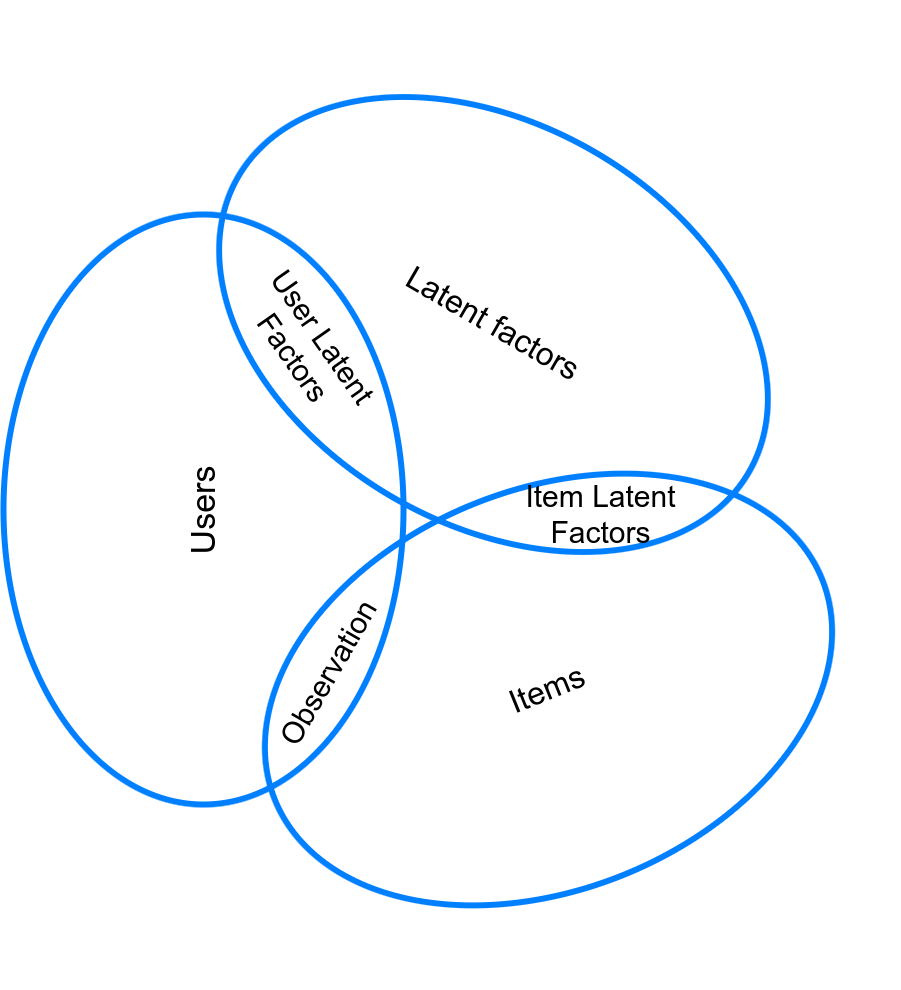
\includegraphics[width=0.5\textwidth]{images/LatentFactors.png}
	\caption{\bfseries LatentFactors}
	\label{LatentFactors}
\end{figure}


\paragraph{} Alternating least squares (ALS) algorithm belongs to the group above. In this case, we assign initially random values of rating between user and items. Then it takes the error between the actual value and the one assigned to it. 
\pagebreak
\paragraph{}Then the algorithm runs again using as input the errors and tries to minimize them. Below we can see a how this algorithm is defined.

\begin{algorithm}
	\caption{ALS for Matrix Completion}\label{ALS}
	\begin{algorithmic}[1]
		\State Initialize X,Y
		\Repeat
		\For{\texttt{u=1...n}}
		\State $x_{u} = (\sum_{r_{ui}}y_{i}y_{i}^{T} + \lambda I_k)^{-1} \sum_{r_{ui}}r_{ui}y_{i} ,\in r_{u*}$
		\EndFor
		\For{\texttt{i=1...m}}
		\State $y_{i} = (\sum_{r_{ui}}x_{u}x_{u}^{T} + \lambda I_k)^{-1} \sum_{r_{ui}}r_{ui}x_{u} ,\in r_{*i}$
		\EndFor
		\Until {convergence}
	\end{algorithmic}
\end{algorithm}

\paragraph{}As we can see above, this algorithm has a $\lambda$ parameter used for normalization during the process. We can see the difference below where we have both the expression with and without normalization factor.

\paragraph{} ALS is a very efficient recommender algorithm. Due to its nature, it can be easily parallelized reducing the execution time needed \cite{DistributedAlgorithmsAndOptimization:4}. It also requires no meta-data about any user or item. Although, ALS suffers from the cold start problem.

\begin{equation}
	\min_{X,Y} \sum_{r_{ui}observed}(r_{ui}-x_{u}^{T}y_{i})^{2}
\end{equation}

\begin{equation}
	\min_{X,Y} \sum_{r_{ui}observed}(r_{ui}-x_{u}^{T}y_{i})^{2} + \lambda(\sum_{u}||x_{u}||^2 + \sum_{i}||y_{i}||^2)
\end{equation}

\paragraph{} Moving forward this thesis, we are going to discuss how those two algorithms were implemented and validate the results they gave.
	\section{Our Experiment}
\subsection{Infrastructure}
\subsubsection{Apache Spark}
The last decade, analyzing big data is at its peek. Lots of data are produced and the need for getting information from them is raised. The most common technique to do this is map-reduce.

Spark's predecessor, hadoop map reduce, was for a long time at its peak.
 Hadoop map reduce, is a distributed map-reduce system, 
this means that it has a mechanism to distribute work on nodes 
and a common interface for handling data. In hadoop's case this was able
 to happen due to Apache hadoop yarn and the HDFS (hadoop distributed file system).
 When a job was scheduled, data were loaded by the hdfs to a worker, 
then the worker was putting the result back to the hdfs. 
Map-reduce is a method that is around a lot time for handling large amounts of data. It has two basic processes, Map which is responsible for turning the data into key value pairs, and Reduce which takes those pairs and turns them into valuable data.

As mentioned in \cite{ibmMapReduce:5}, "The term MapReduce actually refers to two separate and distinct tasks that Hadoop programs perform. The first is the map job, which takes a set of data and converts it into another set of data, where individual elements are broken down into tuples (key/value pairs). The reduce job takes the output from a map as input and combines those data tuples into a smaller set of tuples. As the sequence of the name MapReduce implies, the reduce job is always performed after the map job."

If we would like to see where in the DIKW (Data Information Knowledge Wisdom) stack those processes belong, the map would start with data and the reduce will end up with information.\\

\begin{figure}[h]
	\centering
	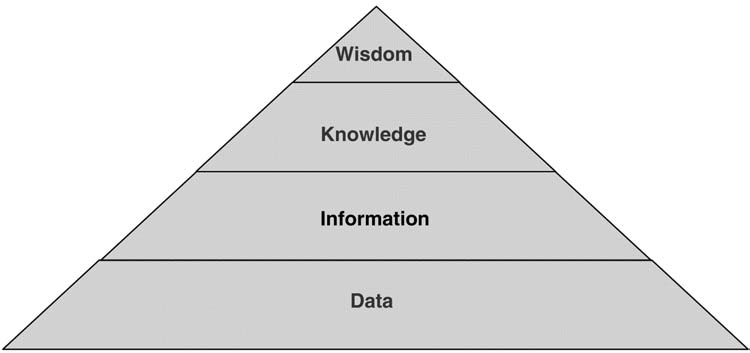
\includegraphics[width=0.5\textwidth]{images/DIKW.png}
	\caption{\bfseries Data Information Knowledge Wisdom Pyramid \cite{TheWisdomHierachy:7}}
	\label{dikw}
\end{figure}

Hadoop was the core map-reduce framework the last years.
As it is described in \cite{Hadoop:9}, and shown in the figure \ref{hadoopStack} hadoop uses hadoop yarn in order to coordinate which process will run on which machine. Also it uses the HDFS (Hadoop Distributed File System) in order to have a common reference for the files over the network. Last but not least, hadoop ecosystem is supported by the Hadoop Commons library. 

\begin{figure}[h]
	\centering
	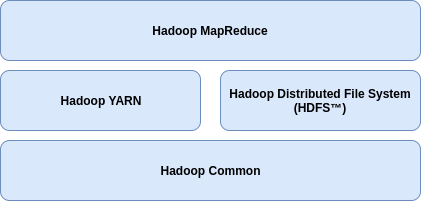
\includegraphics[width=0.5\textwidth]{images/hadoop-stack.png}
	\caption{\bfseries Hadoup Software Stack}
	\label{hadoopStack}
\end{figure}

 In 2009 UC Berkley developed spark \cite{DatabricsSpark:8}.
Spark's predecessor, hadoop map reduce, was for a long time at its peak. Hadoop map reduce, is a distributed map-reduce system, this means that it has a mechanism to distribute work on nodes and a common interface for handling data. In hadoop's case this was able to happen due to Apache hadoop yarn and the HDFS (hadoop distributed file system). When a job was scheduled, data were loaded by the hdfs to a worker, then the worker was putting the result back to the hdfs. 

\paragraph{}Apache spark is the new trend on distributed computation and map-reduce. 
But first things first, what is map-reduce? \\
apache mesos -> data center operating system, references
\\
But innovation knocked the door and resilient distributed datasets entered the room. In spark world, data are loaded to hdfs as before. Then spark loads them in an RDD, this means that data are now accessible on each machine's memory. Any transformation done to a RDD results a RDD, and so forth. After all the transformations are done, spark can transform the results to a file in hdfs.

\begin{figure}[ht]
  \centering
    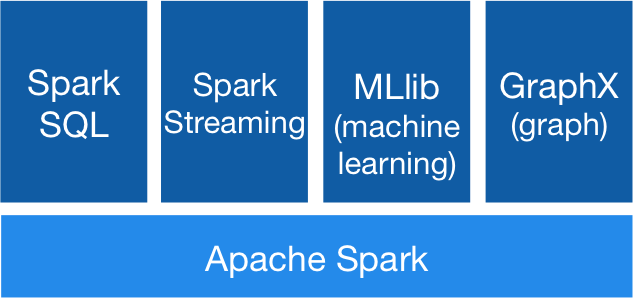
\includegraphics[width=0.5\textwidth]{images/spark-stack.png}
    \caption{\bfseries Apache spark stack \cite{ApacheSpark:1}}
   \label{apacheSparkStack}
\end{figure}

How spark differentiates from its predecessors\\
Spark lightweight in memory data transformation 
Resilient Distributed Datasets (RDDs) \\
mllibs\\
add spark jira note \\\\
Important note: mention als distributed broadcasting implementation. 
\\\\
broadcasting rdd \\
//cite the mastering apache spark book
\cite{ApacheSpark:1} \\
a Spark cluster to be created on AWS EC2 storage.\\
New trends on spark https://github.com/apache-spark-on-k8s/spark cite this repository too.
\subsection{Dataset}
What is the dataset about. This dataset contains users, movies and the rating user made about the movies.
This dataset is splited to multiple subsets of 80000 training sets and respective 20000 reviews.
\cite{MovieLens:3}

\subsection{Implementation and assumptions}
\subsection{Metrics}
\subsubsection{Mean Absolute Error}
As metrics are commonly used the MSE, RMSE and MAE. Due to the fact that the author prefers the last one, MAE was used in this experiment.
\begin{equation}
MAE = \frac{\sum_{i=1}^{n}{|y_{i}-x_{i}|} }{n} = \frac{\sum_{i=1}^{n}\sqrt{{(y_{i}-x_{i})}^{2}}}{n}
\end{equation}
\subsubsection{Execution Time}
Time is measured in milliseconds.
Execution time is always a measure when we are comparing algorithms. Even more if those algorithms execution time is heavily dependent to their complexity.

	\section{Results}
\begin{table}[ht]
		\caption {\bfseries Content Based Algorithm Results}
\begin{tabular}{l|l|r|r}%
   	\bfseries Training Dataset & \bfseries Testing Dataset & \bfseries Mean Absolute Error & \bfseries  Execution time (ms)% specify table head
   	\csvreader[head to column names]{data/contentBased.csv}{}% use head of csv as column names
   	{\\\hline \trainingSet & \testingSet & \MAE & \ExecutionTime}% specify your coloumns here
\end{tabular}
  \label{tab:Content Based Algorithm Results}
\end{table}

\pgfplotstableread[col sep=comma]{data/contentBased.csv}\latentFactorsDataTable
\begin{tikzpicture}
\begin{axis}[
title={Content Based - Mean Absolute Error},
xlabel= Dataset,
ylabel=Mean Absolute Error,
width=1\linewidth, 
xtick=data,
xticklabels from table={\latentFactorsDataTable}{trainingSet}]
\addplot [ybar, fill=blue] table [x expr=\coordindex, y=MAE, col sep=comma] {data/contentBased.csv};
\end{axis}
\end{tikzpicture} \\ \\
\begin{tikzpicture}
\begin{axis}[
title={Content Based - Execution Time},
xlabel= Dataset,
ylabel=Execution Time,
width=1\linewidth, 
xtick=data,
xticklabels from table={\latentFactorsDataTable}{trainingSet}]
\addplot [ybar, fill=blue] table [x expr=\coordindex, y=ExecutionTime, col sep=comma] {data/contentBased.csv};
\end{axis}
\end{tikzpicture}


\begin{table}[ht]
		\caption{\bfseries Latent Factors Algorithm Results}
\begin{tabular}{l|l|r|r}%
	\bfseries Training Dataset & \bfseries Testing Dataset & \bfseries Mean Absolute Error & \bfseries  Execution time (ms)% specify table head
	\csvreader[head to column names]{data/latentFactors.csv}{}% use head of csv as column names
	{\\\hline \trainingSet & \testingSet & \MAE & \ExecutionTime}% specify your coloumns here
\end{tabular}
  \label{tab:Latent Factors Algorithm Results}
\end{table}

\pgfplotstableread[col sep=comma]{data/latentFactors.csv}\latentFactorsDataTable
\begin{tikzpicture}
\begin{axis}[
title={Latent Factors - Mean Absolute Error},
xlabel= Dataset,
ylabel=Mean Absolute Error,
width=1\linewidth, 
xtick=data,
xticklabels from table={\latentFactorsDataTable}{trainingSet}]
\addplot [ybar, fill=blue] table [x expr=\coordindex, y=MAE, col sep=comma] {data/latentFactors.csv};
\end{axis}
\end{tikzpicture} \\ \\
\begin{tikzpicture}
\begin{axis}[
title={Latent Factors - Execution Time},
xlabel= Dataset,
ylabel=Execution Time,
width=1\linewidth, 
xtick=data,
xticklabels from table={\latentFactorsDataTable}{trainingSet}]
\addplot [ybar, fill=blue] table [x expr=\coordindex, y=ExecutionTime, col sep=comma] {data/latentFactors.csv};
\end{axis}
\end{tikzpicture}
	\newpage
\section{Conclusion}
\paragraph{}Recommender systems have a short but intense history. It started from simple statistical models and nowadays it is a great field of study. Recommender systems are now used widely in the online market. Every day you are using them without even noticing it. While you are browsing videos or the web, getting a message from a friend or even listening to music a recommender system might serve you at the time.

\paragraph{} In this last chapter of this thesis, we will summarize the experiment and the result we got. This thesis is the attempt of the author to compare two recommender algorithms. Those algorithms were the classic content based and the alternative least squares. The first one is in the area of collaborative filtering while the other is in the latent factors area.

\paragraph{} Those two algorithms were implemented or used in Apache Spark. The first, the content based algorithm was implemented, the second one the alternating least squares was used via Apache Spark's MLlib library.

\paragraph{} Then those systems were put to test. As metrics were used the mean absolute error(MAE), the root mean square error (RMSE), the ratio between them (MAE/RMSE) and the execution time. Execution time is composed of two parts, the training time and the time taken to make the metrics. Because the metrics are common, on the same platform and they were using the same code, we can assume that the execution time difference has the training part and the prediction part for every rate in the test dataset.

\paragraph{} During the results examination, as it was shown in the previous chapter, we found that the ALS system outperformed the content based on every metric we used. It showed low error metrics, MAE and RMSE, while execution time was low. The ratio MAE/RMSE was high. The last showed us that ALS has fewer data spikes comparing to the content based.

\paragraph{} Recommender systems will be around for quite a long time, it is important to know how to compare them. Even more important is to identify which recommender algorithm to use for each business case.

\paragraph{} This thesis was a very important milestone for the author. This milestone couldn't be true without the help of those mentioned in the acknowledgment page.
\\
\paragraph{Vasileios Simeonidis, \\ August 15, 2017}


%\section*{Acknowledgements}
%This work couldn't be completed without the great support I received from so many people over this year. I would like to thank the following people.
%
%My supervisor Dr. Dimosthenis Kyriazis for totally supporting me in the choices I made and giving me the freedom I was needing.
%
%My friend and fellow student Dimitris Poulopoulos for helping me understand the field of recommender systems and supported me technically and theoretically.
%
%My friends and colleagues George Adamopoulos and Nikos Silvestros for constantly teaching me high-level engineering and scientific thinking. Also, I would like to thank them for putting the right amount of pressure on me in order to complete this thesis.
%
%Kronos, the development team I am part of and helping me to keep my spirit high. Thank you, Apostolos Chissas, Kostas Rigas, Christos Grivas, Peter Lengos, Vasiliki Giamarelou, Maria Karkeli, Eleni Karakizi, Spyros Argyroiliopoulos, Nikos Anagnostou and Ioannis Koutsileos. 
%
%Last but not least, I would like to thank my close friends and family for bearing me while I was anxious about the completion of this thesis.
	
	\bibliography{paper}
	\bibliographystyle{ieeetr}
\end{document}